\documentclass[a4paper,13pt]{article}
\usepackage[UTF8]{ctex}
\usepackage{amsmath}
\usepackage{mathtools}
\usepackage{amsfonts}
\usepackage{enumitem}
\usepackage{multirow}
\usepackage{sidecap}
\usepackage{graphicx}
\usepackage{caption}
\usepackage{booktabs}
\graphicspath{{images/}}
\usepackage{footnote}
\usepackage{ulem}
\usepackage{tocloft}
\captionsetup{font=footnotesize}
\usepackage{setspace}
\usepackage{geometry}
\geometry{left=2.5cm,right=2.5cm,top=2.5cm,bottom=2.5cm}



\newcommand{\chuhao}{\fontsize{42.2pt}{\baselineskip}\selectfont}
\newcommand{\xiaochu}{\fontsize{36.1pt}{\baselineskip}\selectfont}
\newcommand{\yihao}{\fontsize{26.1pt}{\baselineskip}\selectfont}
\newcommand{\xiaoyi}{\fontsize{24.1pt}{\baselineskip}\selectfont}
\newcommand{\erhao}{\fontsize{22.1pt}{\baselineskip}\selectfont}
\newcommand{\xiaoer}{\fontsize{18.1pt}{\baselineskip}\selectfont}
\newcommand{\sanhao}{\fontsize{16.1pt}{\baselineskip}\selectfont}
\newcommand{\xiaosan}{\fontsize{15.1pt}{\baselineskip}\selectfont}
\newcommand{\sihao}{\fontsize{14.1pt}{\baselineskip}\selectfont}
\newcommand{\xiaosi}{\fontsize{12.1pt}{\baselineskip}\selectfont}
\newcommand{\wuhao}{\fontsize{10.5pt}{\baselineskip}\selectfont}
\newcommand{\xiaowu}{\fontsize{9.0pt}{\baselineskip}\selectfont}
\newcommand{\liuhao}{\fontsize{7.5pt}{\baselineskip}\selectfont}
\newcommand{\xiaoliu}{\fontsize{6.5pt}{\baselineskip}\selectfont}
\newcommand{\qihao}{\fontsize{5.5pt}{\baselineskip}\selectfont}
\newcommand{\bahao}{\fontsize{5.0pt}{\baselineskip}\selectfont}

\begin{document}


%-----标题页-----
%-----Title-----
%%-----论文封面一
\begin{titlepage}

\includegraphics[width=2.5cm]{njuxh}
\parbox[t][0.5cm][t]{\textwidth}{}
\begin{center}
	
\parbox[t][7.2cm][t]{\textwidth}{
\begin{center}

\includegraphics[width=7.5cm]{njuwz}\\
{\bf \Large NANJING UNIVERSITY\\}
\vspace{0.3cm}
{\erhao 本~科~毕~业~论~文\\}
\end{center}
}

\parbox[t][6cm][c]{\textwidth}{
\begin{center}
\fontsize{16pt}{8pt}\selectfont
\begin{tabular}{p{4.5em} p{2em} p{4em} p{2.5em} p{6em}}
院~~~~~~~~系 & \multicolumn{4}{c}{}\\
\cmidrule(r){2-5}\addlinespace[10pt]
专~~~~~~~~业 & \multicolumn{4}{c}{}\\
\cmidrule(r){2-5}\addlinespace[10pt]
题~~~~~~~~目 &  \multicolumn{4}{c}{}\\
\cmidrule(r){2-5}\addlinespace[10pt]
年~~~~~~~~级 &  \multicolumn{2}{c}{~~~~~~~~~~~~~} & 学号 & \\
\cmidrule(r){2-3} \cmidrule(r){5-5}\addlinespace[10pt]
学生姓名 & \multicolumn{4}{c}{}\\
\cmidrule(r){2-5}\addlinespace[10pt]
指导教师 & \multicolumn{2}{c}{} & 职称 & \\
\cmidrule(r){2-3} \cmidrule(r){5-5}\addlinespace[10pt]
\multicolumn{2}{l}{论文提交日期} & \multicolumn{3}{c}{}\\
\cmidrule(r){3-5}
\end{tabular}
\end{center}
}

%-----论文封面二
\newpage
 \parbox[t][16cm][t]{\textwidth}{
\begin{center} 
\end{center} 
}
          
\parbox[b][10em][b]{\textwidth}{ \sanhao                                                                  
\begin{tabular}{l p{12em}}
学~~~~~~~~~~~~~~~~号:& {\bf ~~~~}\\
论文答辩日期:& ~~~~~~~~~~年~~~~~~~月~~~~~~~日\\
指~~~导~~~教~~~师: &~~~~~~~~~~~~~~~~~~~~~~(签字)\\
\end{tabular}
}   
\end{center}

%-----中文摘要-----
\end{titlepage}
%\newpage
%-----目录-----
\begin{center}
\sanhao \bf 目录
\end{center}
\contentsline {section}{\sihao \numberline {1}基本介绍}{2}
\vspace{0.5cm}
\contentsline {subsection}{\sihao \numberline {1.1}什么是词嵌入}{2}
\vspace{0.5cm}
\contentsline {subsection}{\sihao \numberline {1.2}之前的工作}{2}
\vspace{0.5cm}
\contentsline {subsection}{\sihao \numberline {1.3}本文的工作}{4}

\contentsline {section}{\sihao \numberline {2}理论分析}{5}
\vspace{0.5cm}
\contentsline {subsection}{\sihao \numberline {2.1}模型介绍}{5}
\vspace{0.5cm}
\contentsline {subsection}{\sihao \numberline {2.2}分布的选取}{6}

\contentsline {section}{\sihao \numberline {3}词表示学习}{8}
\vspace{0.5cm}
\contentsline {subsection}{\sihao \numberline {3.1}学习过程}{8}
\vspace{0.5cm}
\contentsline {subsection}{\sihao \numberline {3.2}实验设置}{9}
\vspace{0.5cm}
\contentsline {subsection}{\sihao \numberline {3.3}结果及分析}{10}
\contentsline {paragraph}{模型及超参数的选择}{10}
\contentsline {paragraph}{两种度量得到的结果}{10}
\contentsline {paragraph}{词义相似度评价}{11}
\contentsline {section}{\sihao \numberline {4}上下位关系的学习}{11}
\vspace{0.5cm}
\contentsline {subsection}{\sihao \numberline {4.1}学习过程}{11}
\vspace{0.5cm}
\contentsline {subsection}{\sihao \numberline {4.2}实验设置}{13}
\vspace{0.5cm}
\contentsline {subsection}{\sihao \numberline {4.3}结果及分析}{14}
\contentsline {paragraph}{边际 $\varepsilon $ 、$\varepsilon ^{'}$的选取对于结果的影响}{14}
\contentsline {paragraph}{迭代次数对实验的影响}{14}
\contentsline {paragraph}{两种模型的对照实验}{14}
\contentsline{section}{\sihao \numberline {5} 结论与展望}{24}
\newpage
\begin{spacing}{1.5}\xiaosi 
\section{基本介绍}
\subsection{什么是词嵌入}
词嵌入(word embedding),是一种稠密的词的分布表示方式,不同于传统的符号表示和词袋模型(bag of words)利用词-上下文共现矩阵(word-context matrix)的稀疏表示,而是将词汇映射到一个连续的希尔伯特空间进行表示。基于语言学家Zellig Haris的假设“在相近的上下文中出现的词汇具有相近的语义”\cite{harris1954distributional}进行训练,使得相近语义表现为希尔伯特空间中某种度量意义下的接近。

分布式的表示方式的最大优点是易于进行计算,尤其是非常适合作为神经网络的输入层,因而被广泛的应用到一系列自然语言处理的具体任务中,包括信息检索\cite{manning2008introduction},问答系统\cite{tellex2003quantitative},主题命名识别\cite{turian2010word}和语义解析\cite{socher2011parsing}等,并取得了非常好的效果。随着近几年来深度学习(deep learning)技术在自然语言处理领域得到广泛运用,对于词嵌入和更广泛的词表示学习成为这几年的研究热点。

\subsection{之前的工作}
之前有大量的关于词嵌入方面的工作,绝大多数是基于向量的表示形式。从方法大致分为显示矩阵分解法、神经网络法和隐式矩阵分解法。

显示矩阵分解法(Explicit Matrix Factorization Methods)是一种传统的获得隐层空间的向量表示的方法.其中经典的工作是隐语义分析法(LSA, Latent Semantic Analysis),通过对term-doc 矩阵进行近似分解(SVD)的手段获得document的topic分布. 对于词分布表示而言,类似的工作是Hypersapce Analogue to Language(HAL)\cite{lund1996producing},通过分解term-term矩阵,即单词和在每个上下文单词出现的词数构成的矩阵,获得词的分布表示。由于这种方法存在着受高频词影响过大的的缺陷(诸如the, and, with等停用词),后续的研究表明通过分解PPMI矩阵(positive pointwise mutual information)是更好的替代方案\cite{lebret2013word}。

另外一种方法是通过从上下文预测中心词的办法学习词的分布表示,通过浅层神经网络学习预测任务来获得词所对应的向量。Bengio在2003年提出用神经网络训练语言模型成功获得了高质量的词向量\cite{bengio2006neural},同过神经网络学习如下条件概率:

\begin{align*}
&x=(C(w_t-1),C(w_t-2),...,C(w_t-n+1))\\
&y=b+Wx+Utanh(d+Hx)\\
&\hat{P}(w_t|w_t-1,...,w_t-n+1)=\frac{e^{y_{w_t}}}{\Sigma_{i}e^{y_i}}
\end{align*}
由于输入层采取concentration的方法处理输入的窗口词表示,对窗口大小的可扩展性较差,并且正则化需要大量的计算,在面对大规模语料的时候效率并不高。后续的工作大多在提高这一框架的性能上展开。

2013年Thomas Mikolov提出了一个更为简单迅速的训练词向量的框架Word2Vec\cite{mikolov2013efficient},采用单层神经网络,通过计算
$w_i^{\prime{}}w_j$来训练得到联合概率$p(w_i,w_j)$。Word2Vec包括CBOW和skip-gram两种计算方式(Figure\ \ref{fig:w2v}),同时也利用了Hierarchical Softmax和Negative Sampling两种快速的正则化方法取代了Bengio的Softmax方法。至此快速获得高质量的词向量成为可能,也使得神经网络在自然语言处理任务中得到普及。随后提出的Glove模型\cite{pennington2014glove}和Swivel模型\cite{shazeer2016swivel}则在Word2Vec的基础上进一步地提升了词向量的训练速度和质量。
\begin{figure}[h]
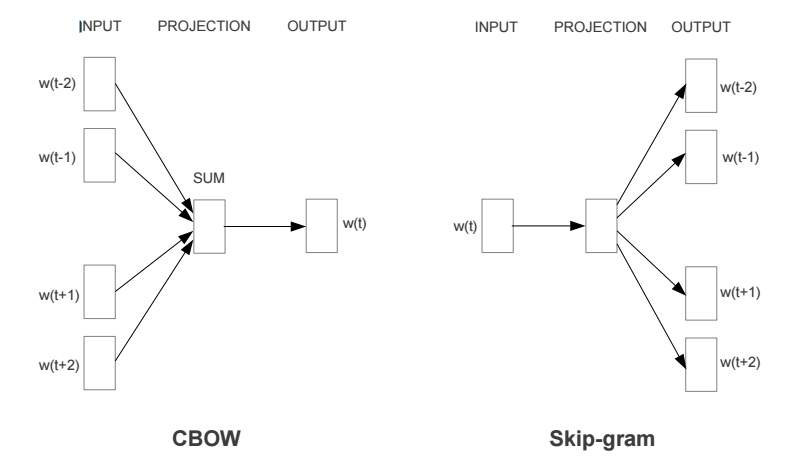
\includegraphics[width=\textwidth,height=8cm]{aaa.jpg}
\caption{\wuhao CBOW模型和skip-gram模型的大致框架}
\centering
\label{fig:w2v}
\end{figure}

大量的实验表明,上述两类取得词向量的方法在语料足够大的情况下在得到词向量的质量上并没有绝对的优劣。2014年Omer Levy等人更是证明了两类方法在数学上的统一性\cite{levy2014neural},即Word2Vec中的SGNG(Skip-Gram with Negative Sampling)等价于分解word-context的PPMI矩阵。随后在O.Levy于TACL发表的\cite{levy2015improving}一文中总结了目前位置常用的训练词嵌入的方法,将Word2Vec模型、Glove模型划分为了隐式矩阵分解方法(Implicit Matrix Decomposition Methods),并通过大量的对照实验,认为相比模型中超参数的调整,上述两种矩阵分解模型的优劣很小,对于参数的控制要重于对模型架构和优化算法的研究。

此后的工作更多地专项词向量的细化工作,比如词向量可解释性的研究,在词向量的训练中引入语言学的一些数据集和监督学习的方法,非英语的词向量研究(比如运用在汉语和日语上的词向量)等。

\subsection{本文的工作}
从之前的工作中可以看出,词的向量表示已经得到了比较成熟的研究,并取得了广泛应用。然而单纯从表示方式上来说,词的向量表示也存在一些不足:1.只用向量空间中的一个点表示词,会造成相当的语义损失,实际上各国语言的词汇中都普遍存在一词多义的现象,向量表示并不能刻画这种不确定性。2.词向量的度量方式比较单一,不论是欧氏距离还是余弦距离,只能用来刻画语义的接近程度,对于语言学中其他语义关系,诸如上下位词(hypernym-hyponym)的刻画比较无力。因而最近关于词的分布式表示的研究,有许多致力于建立更具有语言学解释性,能够包含更多人工抽象的词汇信息(fine-grained lexical resources)的表示模型。

Luke Vilins等人在ICLR 2015中发表的Word Representation Via Gaussian Embedding\cite{vilnis2014word}文章中,提出了一种新的词的分布表示的形式---不同以往的词向量表示,而是试图将词表示成一种特定的分布(以下简称词分布)。词分布通过通常含有一组参数表示分布的均值,这包含了词向量所涵盖的信息。此外,通过模型学习到的分布的其他参数,诸如方差等,提供了词的其他语义信息,诸如词义的不确定程度等,可以作为新的特征运用在具体的自然语言处理任务中。(图\ \ref{fig:w2d})

\begin{SCfigure}
	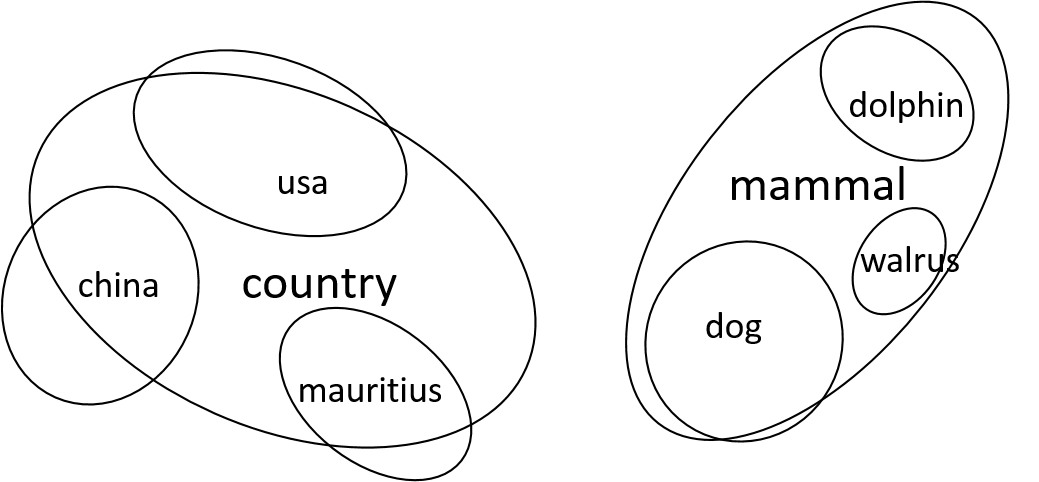
\includegraphics[width=0.7\textwidth]{word2gauss_illustrate.png}
	\caption{\wuhao 词分布的示意图。这里选取的是选择高斯分布对词进行表示的情况。本图表现出了这种表示的两个特点:具有相近词义的分布的均值比较接近;词频较大和词义较宽泛的协方差较大。}
	\centering
	\label{fig:w2d}
\end{SCfigure}

然而囿于篇幅,Vilins等人的文章对于词分布的讨论并不是非常充分,除了他们在future work的环节提出的一些待探索的课题同时,也比较缺乏充分的实验探究。本文正是基于这些问题对词分布这一新颖的表示方式做更深入的讨论。本文的工作将分成三个部分。第一部分针对原文中对于“还有那些分布可以用于表示”尝试作出一些回答,并指出原文中作者设想的student's\ t分布并非是一个很好的选择。第二部分是对于词分布模型在词的相似度等实验上的表现,特别指出了一些超参数的选择会极大影响实验的结果。第三部分则针对原文作者提出的对于非对称关系学习的实验上的补充,并指出原文作者设想的学习这种关系的方法的效果不佳,最后给出自己的修改过的模型和学习策略。

\section{理论分析}

\subsection{模型介绍}

我们将语料经过tokenize得到的一个词典记为$\mathcal{D}$,其中的每一个单词记为$w$,自然有$w\in\mathcal{D}$
。通过设定窗口(window)的大小(记为$i$),对于语料中位置为$n$的词$w_n$,我们把$w_n-i,...,w_n-1,w_n+1,...,w_n+i$称
作上下文词,把所有上下文词的几何记为$\mathcal{C}$,该集合中的每一个词记为$c$,显然$c\in\mathcal{C}$
。一般情况下,我们有$\mathcal{C}\subseteq\mathcal{D}$。对于下文中关于单词和上下文词的表示,我们同样分别以
$w$和$c$来表示以简化表达。

对于一个单词-上文词对样本$(w_i,c_j)$,我们把$c_j$在语料中出现在$w_i$的窗口词对样本称为正样本(positive),反之则称为负样本(negative)。考虑到各种词对样本出现的频率差异很大,单纯的二分类问题并不能很好的建立模型,为此我们引进能量函数(energy function)来给词对样本打分。

设输入为$x$,输出为$y$,我们定义能量函数为$E_\theta(x,y)$,其中$\theta$为能量函数的参数。能量函数只取非负值,其值越大,则意味着该样
本$(x,y)$更“正”,在训练词分布的模型中,即意味着词对样本在语料中出现的概率更大。通过对模型的目标函数进行优化,学习得到的参数$\theta$,即为$x$和$y$的分布表示。以Word2Vec的SGNS模型为例,其优化的能量函
数为
\begin{align*}
E(w,c)=\sigma(w^{\prime{}}c)\cdot\prod_k\sigma(w^{\prime{}}c_N^k)
\end{align*}

其中$\sigma(x)=\frac{1}{1+e^(-x)}$为sigmoid函数,便可以看做以sigmoid函数作为其能量函数。
为了很好的区分正样本和负样本,我们考虑引入排序损失函数(ranking loss function)。设$\mathcal{L}(w,c,c_n)=max(0,\varepsilon-E(w,c)+E(w,c_n))$,$\varepsilon$为正样
本和负样本的一个边界(margin)。当$\varepsilon-E(w,c)+E(w,c_n)>0$即$E(w,c)-E(w,c_n)>m$时小损失函数,从而使得$E(w,c)$和$E(w,c_n)$的差值大于$\varepsilon$。

相对于以往以向量为基础的词分布表示,本文讨论的模型希望将词表示为一个特定的分布,因而需要选取适合与计算分布间的能量函数。Vilins等在ICLR15的文章中,选择了概率乘积核(probability product kernel)和KL散度(Kullback-Leibler divergence)进行建模(以下分别简称为IP能量函数和KL能量函数)。IP能量函数在所有连续分布构成的$\mathcal{L}^2$空间中相当于内积,而KL能量函数则是信息论中常用的度量。下面以高斯分布为例进行说明。

对任何一个词$w$,用一个高斯分布$\mathcal{N}(\mu_w,\Sigma_w)$进行表示。对于IP能量函数,有:
\begin{align*}
E(w,c)&=D_KL(\mathcal{N}_w||\mathcal{N}_c)\\
&=\frac{1}{2}(tr(\Sigma_c^{-1}\Sigma_w)+(\mu_c-\mu_w)^{\prime{}}\Sigma_c^{-1}(\mu_c-\mu_w))-d+ln(\frac{det(\Sigma_c)}{det(\Sigma_w)})
\end{align*}
对于KL能量函数,有:
\begin{align*}
E(w,c)&=D_KL(\mathcal{N}_w||\mathcal{N}_c)\\
&=\frac{1}{2}(tr(\Sigma_c^{-1}\Sigma_w)+(\mu_c-\mu_w)^{\prime{}}\Sigma_c^{-1}(\mu_c-\mu_w))-d+ln(\frac{det(\Sigma_c)}{det(\Sigma_w)})
\end{align*}
其中$d$为设定的词分布的的维度。当选取的高斯分布具有一些特殊的条件,诸如协方差矩阵为对角矩阵时,上述两个能量函数还可以得到进一步简化。

\subsection{分布的选取}

从上面的推导可以看到,由于高斯分布良好的性质,两种能量函数都能够得到封闭解(close form)。那么是否存在其他良好的分布函数,适合用作词的向量表示?Vilins在其ICLR15的工作的future work一节曾经提到过可以尝试使用其他分布进行尝试,比如Student’s\ t,然而并没有给出相应的结论,为此我们将针对一些常见的分布进行讨论。
特别要提出的是,分布的选择,以及能量函数的选择对于词的表示效果的影响是比较难以预测的,对于具体选择那种分布,本文更倾向与将易于计算摆在优先考虑的位置,因而具有解析形式的密度函数的一类分布是较优的选择。

首先我们讨论一般椭圆分布(general elliptical distribution)的情况。我们采取\cite{gomez2003survey}中给出的定义,只考虑一类具有解析形式的密度函数的椭圆分布。设$E(\mu,\Sigma,g)$为椭圆分布,且具有密度函数$f(x)$如下:
\begin{align*}
f(x;\mu,\Sigma,g)=c_n|\Sigma|^{-\frac{1}{2}}g((x-\mu)^{\prime{}}\Sigma^{-1}(x-\mu))
\end{align*}
其中$\mu\in\mathbb{R}^n$,$\Sigma$是$n$维正定矩阵,$c_n$是正则项,$g$是一个在$[0,\infty)$上勒贝格可测的非负函数且满足:
\begin{align*}
\int_0^{\infty}t^{\frac{n}{2}-1}g(t)dt<\infty
\end{align*}
我们先考虑两个分布的IP能量函数$E(f_1,f_2)$:
\begin{align*}
E(f_1,f_2)&=c_n^1c_n^2(|\Sigma_1||\Sigma_2|)^{-\frac{1}{2}}\int g_1\cdot g_2(x)dx \\
g_1 \cdot g_2(x)&=g_1((x-\mu_1)^{\prime{}}\Sigma_1^{-1}(x-\mu_1))g_2((x-\mu_2)^{\prime{}}\Sigma_2^{-1}(x-\mu_2))
\end{align*}
关键在于积分$\int g_1\cdot g_2(x)dx$是否存在闭式解。首先将$g(x)$延拓到$(-\infty,\infty)$上的偶函数,则我们得到:
\begin{align*}
\int_{-\infty}^{\infty}g_1(x)g_2(x)dx&=2\int_{0}^{\infty}g_1(x)g_2(x)dx \\
&=\int_{-\infty}^{\infty}g_1(x)g_2(-x)dx
\end{align*}
考虑函数的卷积:
\begin{align*}
g_1\otimes g_2(x)&= \int_{-\infty}^{\infty} g_1(t)g_2(x-t)dt \\
g_1\otimes g_2(0)&= \int_{-\infty}^{\infty} g_1(t)g_2(-t)dt   
\end{align*}
结合(1)(2),我们可以把求积分的解析解转化为求函数卷积的解析解。
对于高斯分布而言,考虑到其在卷积下的不变性质(两个高斯分布的卷积依然是高斯分布),可以通过提取高斯核的技巧求解出解析解。然而对于一般的椭圆分布而言,$g$的选择在可积性的约束下并不能很好的保证其卷积的情况。

以原文章中提到的Student's\ t分布为例,其$g(t)=(1+\frac{x^2}{v})^{-\frac{v+1}{2}}$。关于t分布的卷积计算
\cite{nadarajah2005convolutions}给出了一个可用的结论:当$v_1$和$v_2$皆为奇数时存在解析解,否则不存在解析解。此外,选取t分布作为模型中对词的表示还会引起IP能量函数
的导数难以求解,提高了模型训练的难度,因而高斯分布可以说是一个非常好的选择。

另外一系列常用的分布是指数族分布(exponential family distribution)。指数族分布的密度函数表现为如下形式:
\begin{align*}
p_{\theta}(x)=exp(\mathcal{A}(x)+\theta^{\prime{}}\mathcal{T}(x)-\mathcal{K}(\theta))
\end{align*}
\cite{jebara2004probability}对于指数族分布的IP能量函数计算(即指数族分布的概率乘积核)进行了讨论。对于:
\begin{align*}
k(x,x^{\prime{}})=\int_x p_\theta(x)^{\gamma} p_{\theta^{\prime{}}}(x)^{\gamma}dx
\end{align*}
当$\gamma=1$(probability product kernel)时,只有$\mathcal{A}$和$\mathcal{T}$满足某些特殊的形式
时才具有闭式解。

然而当$\gamma=\frac{1}{2}$时,$k(x,x^{\prime{}})$总能写成如下形式的闭式解:
\begin{align*}
k(x,x^{\prime{}})&=\int_x p_\theta(x)^{\frac{1}{2}} p_{\theta^{\prime{}}}(x)^{\frac{1}{2}}dx \\
&=\int_x exp(\mathcal{A}(x)+(\frac{\theta}{2}+\frac{\theta^{\prime{}}}{2})^{\rm T}\mathcal{T}(x)-\frac{1}{2}\mathcal{K}(\theta)-\frac{1}{2}\mathcal{K}(\theta^{\prime{}})) \\
&=exp(\mathcal{K}(\frac{\theta}{2}+\frac{\theta^{\prime{}}}{2})-\frac{1}{2}\mathcal{K}(\theta)-\frac{1}{2}\mathcal{K}(\theta)-\frac{1}{2}\mathcal{K}(\theta^{\prime{}})) 
\end{align*}
对于$\gamma=\frac{1}{2}$时,$k(x,x^{\prime{}})$被称作巴特查里亚距离(Bhattacharyya distance)。巴氏距离同样
可以表示两个分布的相似程度,在合适的$\mathcal{K}$的选择下我们依然能够的到易于计算的能量函数,至于其与IP能量函数孰优孰劣本文不做展开讨论。

\cite{jordan2003introduction}对于指数族分布的KL散度的计算做出了讨论:
\begin{align*}
D(p \parallel p^{\prime{}}) &= E_p log \frac{p}{p_{\prime{}}} \\
&=E_p (\theta - \theta^{\prime{}})^{T} \mathcal{T}(x) - \mathcal{A}(\theta) + \mathcal{A}(\theta^{\prime{}}) \\
&= (\theta - \theta^{\prime{}})^{T} \mu - \mathcal{A}(\theta) + \mathcal{A}(\theta^{\prime{}})
\end{align*}
其中$\mu = E_p (\mathcal{T}(x))$。由此可见指数族分布在采取巴氏距离的情况下,能量函数有稳定的解析解。对于指数族分布是否适合作为词分布表示,是值得进一步探究的地方。

为了训练的方便,以及专注于讨论模型在具体任务上的问题,本文沿袭前文的做法,统一采用高斯分布作为表示。

\section{词表示学习}

\subsection{学习过程}
根据前面一节的分析,我们采用高斯分布用作词分布的表示,同时为了减少参数的存储空间,我们选择
协方差矩阵为对角矩阵的一类高斯分布,但当协方差矩阵具有别的一些良好性质,尤其是存在一些低阶的
分解的时候也同样适用,这里就不在进一步讨论。

为了进行梯度下降方法,我们需要求解出能量函数关于参数的导数的表达形式,我们分别对IP能量函数和
KL散度两种情况给出计算的结果。

对于IP能量函数而言:
\begin{align*}
E(w,c)=\mathcal{N}(0;\mu_w-\mu_c,\Sigma_w+\Sigma_c)
\end{align*}
为了防止指数函数导致数值过大或过小,我们一般对它的自然对数进行计算,即:
\begin{align*}
log(E(w,c)) = -\frac{1}{2}det(\Sigma_w+\Sigma_c) - \frac{1}{2}(\mu_w-\mu_c)^{T}(\Sigma_w+\Sigma_c)^{-1}(\mu_w-\mu_c) - \frac{d}{2}log(2\pi)
\end{align*}
因而进一步计算其导数:
\begin{align*}
\frac{\partial{}logE(w,c)}{\partial{}\mu_w} &=\frac{\partial{}logE(P_w,P_c)}{\partial{}\mu_c}  =-\Phi_{wc}  \\
\frac{\partial{logE(P_w,P_c)}}{\partial{\Sigma_w}}& =\frac{\partial{logE(P_w,P_c)}}{\partial{\Sigma_c}} = \frac{1}{2}(\Phi_{wc} \Phi_{wc}^{T}-(\Sigma_w+\Sigma_c)^{-1})
\end{align*}
其中$\Phi_{wc} = (\Sigma_w+\Sigma_c)^{-1}(\mu_w-\mu_c)$。
同样,对于KL散度而言:
\begin{align*}
E(w,c)=\mathcal{D}_{KL}(w||c)
\end{align*}
其求导的结果如下:
\begin{align*}
\frac{\partial{}E(w,c)}{\partial{}\mu_w} &= - \frac{\partial{}E(w,c)}{\partial{}\mu_c} =  -\Phi_{wc}^{'} \\
\frac{\partial{}E(w,c)}{\partial{}\Sigma_w} &= \frac{1}{2}(\Sigma_w^{-1} \Sigma_{c} \Sigma_{w}^{-1} + \Phi_{wc})^{'}\Phi_{wc}^{'} - \Sigma_w^{-1} \\ 
\frac{\partial{}E(w,c)}{\partial{}\Sigma_c} &= \frac{1}{2}(\Sigma_c^{-1} - \Sigma_{w}^{-1})
\end{align*}
其中$\Phi_{wc}^{'}=\Sigma_{i}^{-1}(\mu_i-\mu_j)$。

此外还有一些训练中的细节需要注意:为了防止词分布的均值,协方差的数字过大和过小,需要对其作出一些正则化约束。
比如对于协方差而言,可以设定两个超参数$c$,$\mathcal{C}$,使得$\Sigma$满足$cI<\Sigma<\mathcal{C} I$($A>B$表示$A-B$是正定矩阵);
对于KL散度这种非对称的能量函数,在进行negative sampling的时候需要分别对两个位置进行等。

相比前文的工作,本文特别要强调的是,关于协方差矩阵的范围(这里相当于$\Sigma$的最大、最小特征值)的选取,是非常影响结果的,
并在后面的实验评价一节中会特地进行讨论。

\subsection{实验设置}
获得词表示最普遍的做法,是根据语义的上下文假设,本质上是用词对的共现频率作为特征的训练手段。
在自然语言处理的工作中,高质标注数据集的稀缺一直是提高模型性能的一个瓶颈,而这种无监督的训练
方法则可以充分利用互联网产生的大量文本信息,利用海量数据获得良好的训练效果。

适用于词分布的训练的数据集有很多,常用语料库,英文的有维基百科(Wikipedia)、华盛顿邮报(WSJ)、推特(Twitter)等,中文的则有人民日报、微博等。本文采取维基英文百科三月份的镜像进行训练\footnote{\wuhao 可以从https://dumps.wikimedia.org/处下载维基百科各时间点的镜像文件},训练采用了seomoz在github上公开的代码并加以修改。\footnote{\wuhao https://github.com/seomoz/word2gauss/}

\subsection{结果及分析}



\paragraph{模型设置}

为了控制实验参数的规模,本文的实验只保留语料中出现次数大于等于500的单词,并且去除停用词(Stop Words)。基于便于计算的考虑,统一采用对角型协方差矩阵,表示的维度$d$选择为50, 详细的超参数见下表:
\begin{center}
\begin{tabular}{| l | c |}
\hline
\bf initial learning rate & 0.1 \\
\bf margin\footnote{\wuhao margin用于区分正样本和负样本} & 0.1 \\
\bf Negative Sampling number & 5 \\
\bf context window size & 5 \\
\bf iteration & 5 \\
\hline
\end{tabular}
\captionof{table}{\wuhao 词表示实验的超参数设置}
\label{tab:hy}
\end{center}

\paragraph{两种度量得到的结果}
我们分别通过cosine函数和IP能量函数作为衡量词相似度的两个指标,选取最相近的20个词,结果如下表:
\begin{center}
\begin{tabular}{| c | c |}
\hline
\textbf{Query Word(metric)} & \textbf{Neighborhood Words} \\
\hline
math(IP) & theory, mathematics, physics, psychology, geometry \\
\hline
math(cosine) & algebra, arithmetic, calculus, mathematics, coursework \\
\hline
google(IP) & software, internet, youtube, microsoft, iso \\
\hline
google(cosine) & github, gmail, skype, facebook, yahoo \\
\hline
country(IP) & nation, countries, sweden, iceland, belgium \\
\hline
country(cosine) & barbadian, nation, ireland, sweden, kenya \\
\hline 
\end{tabular}
\captionof{table}{\wuhao 词分布表示在两种度量下得到的临近词的结果,其中IP表示用IP能量函数计算相似度,cosine表示用余弦函数只计算均值的相似度。IP能量函数得到的结果按照协方差矩阵的行列式由高到低排列。}

\end{center}
从结果来看两种能量函数获取词相似度的能力相近,可见词分布包含了词向量模型对于词义建模的能力。此外,由于IP能量函数的结果按照协方差矩阵的行列式由大到小排序,可见具有较大行列式的词,如internet,theory,nation,具有交广泛的含义,而较小行列式的词,如geometry,microsoft等,则含义非常具体。

\paragraph{词义相似度评价}
我们使用一些人工构造的数据集来进行词义相似度的评价。每个模型的得分是数据集中两个词的人工打分和模型的出的两个词的相似度的皮尔逊相关系数(Pearson Correlation Coefficient)的百分数。

其中,WordSim-353包含353对单词和它们的相似度得分。这些得分是0\~{}9的数字构成,共计10个人的打分并给出其平均分。Lexsim-999与WordSim-353的构成方式类似,不过具有更多的词对,并且评测比前者要严格。

这里模型的在sigma\_min 和 simga\_max两个关键的超参数上分别取值为0.5和1.0,其余的超参数与表\ref{tab:hy}的设置相同,得到结果如表\ref{tab:sim}:

\begin{center}
\begin{tabular}{| l | c | c | c |}
\hline
\textbf{Dataset} & \textbf{SG \textbackslash 50d} & \textbf{GR \textbackslash 50d \textbackslash cos} & \textbf{GR \textbackslash 50d \textbackslash IP} \\
\hline
WordSim-353 & 59.89 & 58.01 & 42.87 \\
\hline
SimLex-999 & 29.39 & 27.59 & 20.91 \\
\hline
\end{tabular}
\captionof{table}{\wuhao 词相似度测评的结果。SG代表Skip-Gram模型,GR(Gaussian Representation)代表本文中的模型。50d表示维度为50.cos与IP分别指cosine函数和IP能量函数,从数据上看IP能量函数表现词相似度的能力相对较弱}
\label{tab:sim}
\end{center}

\paragraph{超参数的选取}之前的工作中提到词分布表示模型对于一些超参数非常敏感,尤其是协方差的上下界的选取,然而并没有给出相应的实验和取值策略。本文针对这一问题给出了一组实验,其结果见表\ref{tab:sigma}

从结果中看,$\sigma_{min}$取0.5,$\sigma_{max}$取1.0是唯一的同时在大小语料下皆表现出良好效果的选择,其余的实验并不能总结出一个比较好的调参策略。从理论上说,当$\sigma_{min}$和$\sigma_{max}$非常接近时,词分布表示退化成词向量表示,而IP与cosine两种度量的方式应当趋同,当然这样便失去了词分布表示的意义。我们认为这可能是这一表示模型的一个缺点。
\newpage
\begin{center}
\begin{tabular}{| l | l | l | c | c |}
\hline
\bf $\sigma_{min}$ & \bf $\sigma_{max}$ & \bf vocab & \bf similarity(cosine) & \bf similarity(IP) \\
\hline
0.5 & 1.0 & 114186 & \bf 0.581* & \bf 0.437* \\
\hline
0.6 & 1.0 & 114186 & 0.503 & 0.203\\
\hline  
0.7 & 1.0 & 114186 & 0.618 & 0.161 \\
\hline
0.5 & 1.0 & 64617 & 0.544 & 0.385 \\
\hline
0.5 & 1.5 & 64617 & 0.203 & 0.159 \\
\hline
0.3 & 1.2 & 64617 & 0.448 & 0.206 \\
\hline
\end{tabular}
\captionof{table}{\wuhao 
关于$\sigma$的上下界选取对于词义相似度的影响,其中$\mu_{max}=4.0$,我们反复的实验一些组合,只有一组得到了较好的结果,可见这组参数的选取对于实验结果的影响是巨大的}
\label{tab:sigma}
\end{center}

\section{上下位关系的学习}

\subsection{学习过程}

词分布表示相比于其他向量表示模型的最大不同在于,它自然引进了KL散度这一非对称的度量,能够学习一些通过偏序关系形成的层次结构,比如上下位关系、语义的继承关系(entailment)等。ICLR15的论文中,作者指出了该模型具有学习这种层次结构的能力,然而本文则想通过上下位词的学习试图说明原论文的模型学习的效果并不理想,并给出了改进方式和二者的对比实验。

首先解释一下什么是上下位词(hypernym-hyponym)关系。在语言学中,下位词(hyponym)相对于上位词(hypernym),是一种is-a的关系。例如“狗是一种哺乳动物”、“西瓜是一种水果”,“狗”、“西瓜”相对于“哺乳动物”、“水果”是下位词,反之则是上位词。(Figure\ \ref{fig:hyper})上下位词关系的引入对诸如问答系统、自然语言推断(natural language inference)等任务的效果具有很好的提升。

\begin{figure}[h]
	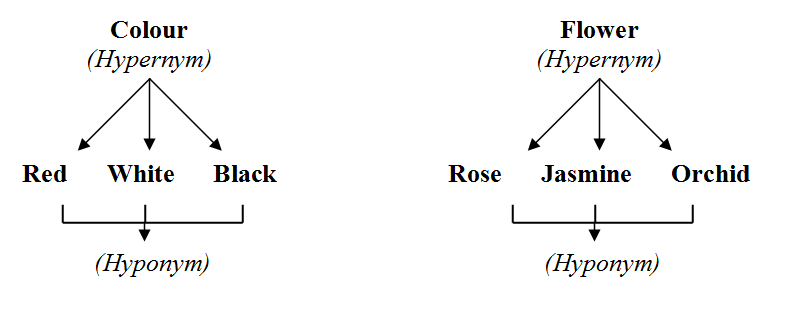
\includegraphics[width=\textwidth]{hypernym-hyponym.png}
	\caption{\wuhao 上下位词的两个例子}
	\centering
	\label{fig:hyper}
\end{figure}

在ICLR15的文章中,作者采用KL散度的能量函数,将具有上下位关系的词对作为正样本,并通过分别对上位词和下位词位置进行负采样得到的词对作为负样本,采用和词表示学习同样的方式进行训练。其损失函数如下:
\begin{align*}
\begin{cases}
Loss(v_{hyper}, v_{hypo}) &= max\{ 0, \varepsilon - D_{KL}(v_{hyper}||v_{hypo}) + D_{KL}(v_{hyper}||v_{neg}) \}  \\
Loss(v_{hyper}, v_{hypo}) &= max\{ 0, \varepsilon - D_{KL}(v_{hyper}||v_{hypo}) + D_{KL}(v_{neg}||v_{hypo}) \}
\end{cases}
\end{align*}

从该损失函数可以看出,存在上下位关系的词对具有较大的KL散度值(本质上是增大上位词的协方差矩阵,减小下位词的协方差矩阵),并且与负样本存在一个边界,这个边界可以通过交叉验证(cross-validation)等手段获得。然而不得不指出的是,这种方式存在这如下的问题:
\begin{enumerate}[label=\alph*)]
\item 负采样的方式不合适。\cite{he2015learning}曾提指出在对知识图谱三元组的两个本体进行负采样时,要使得进行采样的位置尽可能的减少会产生假负样本(false-negative)的情况。这同样适用于对于上下位词的采样。举一个例子:对于上下位词对(mammal.n.01,dog.n.01)对于下位词"dog.n.01"进行采样时,由于其他的哺乳动物都是其下位词,有相当的概率得到的并非负样本。这种采样不正确的情况,会使得处于上位词位置的表示存在过拟合现象(即对任意的词都会判定为存在上下位关系)。从后面的实验部分可以看出,原模型的召回率(Recall)非常高。

\item 损失函数设计的并不合理。实际上,对于一个词对$(w_a,w_b)$而言存在着三种上下位情况(上下位关系记为$\preceq$,下文沿用该记号):$w_a \preceq w_b$、$w_b \preceq w_a$、$w_a$和$w_b$无关系。对于第一种情况的判断,由于KL散度的性质,只要存在$D_{KL}(v_a || v_b) \preceq \varepsilon$即可,然而后两中情况的判断,还需要考虑$D_{KL}(v_b || v_a)$与$\varepsilon$的关系。然而对于原文章中的损失函数而言,单纯的增大正样本和负采样样本之间的边际,有时会造成$D_{KL}(v_hyper||v_neg)$或$D_{KL}(v_neg||v_hypo)$,使得他们产生相反的上下位词的关系。从后面的实验中可以看出,这会造成模型的精准度(Precision)迅速下降。
\end{enumerate}
为了解决这两个问题,本文同样提出了两种应对方法:
\begin{enumerate}[label=\alph*)]
\item 只对上位词位置进行负采样。考虑到这里训练的负样本是不构成上下位词关系的词对,且上下位词呈现的是一种树状的层次结构,下位词的上位词是唯一确定的(相对词义而言,多义词会存在多个)。

\item 考虑新的损失函数:
\begin{align*}
Loss(v_{hyper},v_{hypo}) &= max \{0, \varepsilon - D_{KL}(v_{hyper} || v_{hypo}) + D_{KL}(v_{neg} || v_{hypo})\} \\
                         &+ min \{0, \varepsilon^{'} - D_{KL}(v_{neg} || v_{hypo}) + D_{KL}(v_{neg}^{'} || v_{hypo})\}
\end{align*}
在沿用原模型损失函数的基础上,我们新添加了一个对负样本的正则项和边际,来避免前面b)中出现的问题。这个损失函数同样反映了我们新的判别标准:对于词对$(w_a,w_b)$当$D_{KL}(w_a||w_b)-D_{KL}(w_b||w_a) > \theta$时,认为$w_a \preceq w_b$;当$|D_{KL}(w_a||w_b)-D_{KL}(w_b||w_a) < \theta|$时认为$w_a$和$w_b$无上下位关系。这里的$\theta$同样需要通过交叉验证来选取,不过一般情况下会大于训练时的$\varepsilon$,这一点在后面的实验中会进行讨论。
\end{enumerate}

\subsection{实验设置}

关于上下位词关系最常用的语料库是WordNet\footnote{\wuhao George A. Miller (1995). WordNet: A Lexical Database for English. Communications of the ACM Vol. 38, No. 11: 39-41. }。WordNet是一个英语词汇数据库(lexical database)。区别与常见的词典,WordNet将所有的单词聚成一个同义词集合(synsets)来表示一个共同的语义。为了方便的获得训练集和测试集,本文采用了NLTK\footnote{\wuhao Natural Language Toolkit, a python package to build natural language processing program}的wordNet Interface,获得了所有上下位词关系的传递闭包(transitive closures),共计698587个正样本词对,按一定比例获得训练集和测试集中的正样本,负样本则按照负采样的方法生成。我们这里不对分布的具体选取做出讨论,因此选取均值的维数为50,协方差矩阵为对角型矩阵,迭代次数会在随后的结果中指明,负采样个数统一设定为5。训练集和测试集中正样本的比例为4:1,测试集正负样本比例为1:1

\subsection{结果及分析}

我们将对模型中超参数的选取,本文改进的模型相比原模型的提升进行一些的对比实验。

\paragraph {边际 $\varepsilon$ 、$\varepsilon^{'}$的选取对于结果的影响}

我们设定最后判定结果的$\theta=5$,迭代次数为3,分别考虑改变$\varepsilon$和$\varepsilon^{'}$对于最后结果的情况:
\begin{center}
\begin{tabular}{| c | c | c | c |}
	\hline
	\bf $\varepsilon$,$\varepsilon^{'}$ & \bf Precision & \bf Recall & \bf Accuracy \\
	\hline
	5,0.3 & 0.81720 & 0.78560 & 0.80493 \\
	\hline
	6,0.3 & 0.81710 & 0.79802 & 0.80967 \\
	\hline
	7,0.3 & 0.81592 & 0.80801 & 0.81286 \\
	\hline
	8,0.3 & 0.81410 & 0.81808 & 0.81564 \\
	\hline
	8,0.1 & 0.81317 & 0.82050 & 0.81599 \\
	\hline
	8,0.7 & 0.81617 & 0.81403 & 0.81534 \\
	\hline
	8,1.3 & 0.81759 & 0.81034 & 0.81478 \\
	\hline
\end{tabular}
\captionof{table}{\wuhao 两种margin的选择对于结果的影响}
\end{center}
从实验的结果可以看出,$\varepsilon$越大、$\varepsilon^{'}$越小,模型的Accuracy越高,但总的来说这两个参数的调整对模型的表现影响不大。

\paragraph{迭代次数对实验的影响}
 
我们设定$\theta=3$,$\varepsilon=5$,$\varepsilon^{'}=0.3$,只改变训练集迭代的次数,得到如下结果:
\begin{center}
\begin{tabular}{| l | l | l | l |}
	\hline
	\bf iterations & \bf Precision & \bf Recall & \bf Accuracy \\
	\hline
	3 & 0.71980 & 0.85908 & 0.76233 \\
	\hline
	5 & 0.72693 & 0.86534 & 0.77015 \\
	\hline
	10 & 0.73179 & 0.87426 & 0.77692 \\
	\hline
	20 & 0.73441 & 0.88625 & 0.78287 \\
	\hline
	50 & 0.73752 & 0.90859 & 0.79261 \\
	\hline
\end{tabular}
\captionof{table}{\wuhao 迭代次数对结果的影响}
\end{center}
从实验数据中可以看出,随着迭代次数的增加,模型效果得到显著的提升,从3次到50次迭代性能提高的近3个百分点。由于上下位词的训练集比较小,为了得到高质量的分布,相当的迭代次数是必要的。

\paragraph{两种模型的对照实验}

考虑到不同超参数会影响模型的效果,我们特地选取了多种参数组合进行对照实验,其中本文修改过的模型的$\varepsilon$设定为0.1,得到结果如下:

\begin{center}
\begin{tabular}{| c | c | c | c | c | c | c |}
	\hline
	\bf Implementation & \multicolumn{3}{| c |}{\bf Original} & \multicolumn{3}{| c |}{\bf Modified} \\ \cline{2-7}
	($\varepsilon$,$\theta$,iterations) & Precision & Recall & Accuracy & Precision & Recall & Accuracy \\ 
	\hline
	5,3,10 & 0.63007 & 0.94993 & 0.69610 & 0.73033 & 0.87629 & \textbf{0.77636*} \\
	\hline 
	5,3,50 & 0.64172 & 0.96508 & 0.71313 & 0.73722 & 0.91044 & \textbf{0.79296*}  \\
	\hline
	7,5,10 & 0.70720 & 0.93409 & 0.77367 & 0.81485 & 0.82856 & \textbf{0.82015*}  \\
	\hline
	7,5,50 & 0.70627 & 0.95981 & 0.78032 & 0.81912 & 0.88460 & \textbf{0.84477*}  \\
	\hline
\end{tabular}
\captionof{table}{\wuhao 模型对比实验}
\end{center}

可以看出,我们修改后模型的结果在相同的参数设置下要优于原模型。原模型的召回率远高于精准率,验证了之前对其对正样本过拟合的推断。

\section{结论和展望}
在作者原先工作的基础上,本文对词分布表示这一新的表示方式做了理论和实验上的探究。在理论分析一节中,我们论证了用于表示的分布不仅限于高斯分布一种情况,其他分布对于词表示是否具有更好的效果,这是一个值得探究的方向,比如本文中提出的指数族分布和巴氏距离,可以构建一个新的表示方法。

词分布表示最引人瞩目的地方在于其对于非对称关系的学习能力。不需要想向量表示模型那样自己构造非对称度量,KL散度的自然引进不仅便于计算,具有很好的可解释性。实际上不光是对于上下位词这种非对称关系的学习,目前已经有一些工作将这一模型运用到句子的蕴含关系(entailment),知识图谱(Knowledge Graph)的本体-关系的学习等其他任务上去,并取得了很好的效果。

然而词分布模型仍然存在一些待改进的问题:
\begin{enumerate}
	\item 对于词义的学习效果不算很好
从词表示学习一节的实验中可以看出,相对于以前向量表示模型对于词义相似度的学习效果,词分布模型并不存在优势,在IP能量函数这一度量下甚至存在一定差距,这导致该模型在一些依赖词义相似度的任务中可能并没有太大优势。

	\item 协方差学习到的信息不明确
相比向量表示模型,词分布模型学习得到的协方差如何利用是一个问题。从实验结果可以看出协方差一定程度上反映除了词的多义性和抽象性,然而通过IP能量函数将协方差引入词义相似度的评测时,并没有取得优于向量表示的结果。如何理解和利用协方差学到的信息,并将其作为表示结合到目前的一些算法框架中仍然有待探究。最近利用协方差关于多义性的反映,用来通过混合高斯模型学习词的多义表示(multi-prototype)的任务是在这一方面很好的探究。
\end{enumerate}

\end{spacing}
\newpage
\bibliographystyle{plain}
\bibliography{MyBib}

\end{document}